\documentclass[a4paper, 10pt, ]{article}

\usepackage[slovak]{babel}

% ------------------------------

\usepackage[utf8]{inputenc}
\usepackage[T1]{fontenc}

\usepackage[left=4cm,
            right=4cm,
            top=2.1cm,
            bottom=2.6cm,
            footskip=7.5mm,
            twoside,
            marginparwidth=3.0cm,
            %showframe,
            ]{geometry}

\usepackage{graphicx}
\usepackage[dvipsnames]{xcolor}
% https://en.wikibooks.org/wiki/LaTeX/Colors

% ------------------------------

\usepackage{lmodern}

\usepackage[tt={oldstyle=false,proportional=true,monowidth}]{cfr-lm}
% https://mirror.szerverem.hu/ctan/fonts/cfr-lm/doc/cfr-lm.pdf

% ------------------------------

\usepackage{amsmath}
\usepackage{amssymb}
\usepackage{amsthm}

\usepackage{booktabs}
\usepackage{multirow}
\usepackage{array}
\usepackage{dcolumn}

\usepackage{natbib}

% ------------------------------

\hyphenpenalty=6000
\tolerance=1000

\def\naT{\mathsf{T}}

% ------------------------------

\makeatletter

    \def\@seccntformat#1{\protect\makebox[0pt][r]{\csname the#1\endcsname\hspace{4mm}}}

    \def\cleardoublepage{\clearpage\if@twoside \ifodd\c@page\else
    \hbox{}
    \vspace*{\fill}
    \begin{center}
    \phantom{}
    \end{center}
    \vspace{\fill}
    \thispagestyle{empty}
    \newpage
    \if@twocolumn\hbox{}\newpage\fi\fi\fi}

    \newcommand\figcaption{\def\@captype{figure}\caption}
    \newcommand\tabcaption{\def\@captype{table}\caption}

\makeatother

% ------------------------------

\usepackage{fancyhdr}
\fancypagestyle{plain}{%
\fancyhf{} % clear all header and footer fields
% \fancyfoot[C]{\sffamily {\bfseries \thepage}\ | {\scriptsize\oznacenieCasti}}
\fancyfoot[C]{\sffamily {\bfseries \thepage}{\color{Gray}\scriptsize$\,$z$\,$\pageref{LastPage}}\ | 
\includegraphics[height=5pt]{../../COMMONFILES/KUT_logo_v0.1.pdf}{\scriptsize\KUTporadoveCislo}}
\renewcommand{\headrulewidth}{0pt}
\renewcommand{\footrulewidth}{0pt}}
\pagestyle{plain}

% ------------------------------

\usepackage{titlesec}
\titleformat{\paragraph}[hang]{\sffamily  \bfseries}{}{0pt}{}
\titlespacing*{\paragraph}{0mm}{3mm}{1mm}
\titlespacing*{\subparagraph}{0mm}{3mm}{1mm}

\titleformat*{\section}{\sffamily\Large\bfseries}
\titleformat*{\subsection}{\sffamily\large\bfseries}
\titleformat*{\subsubsection}{\sffamily\normalsize\bfseries}


% ------------------------------

\PassOptionsToPackage{hyphens}{url}
\usepackage[pdfauthor={},
            pdftitle={},
            pdfsubject={},
            pdfkeywords={},
            % hidelinks,
            colorlinks=false,
            breaklinks,
            ]{hyperref}


% ------------------------------

\graphicspath{%
{../fig_standalone/}%
{../../PY/fig/}%
{../../ML/fig/}%
{./fig/}%
}

% ------------------------------

\usepackage{enumitem}

\usepackage{lettrine}

% ------------------------------

\usepackage{lastpage}

\usepackage{microtype}

% ------------------------------

\usepackage{algorithm}
\usepackage[noend]{algpseudocode}
\makeatletter
\renewcommand{\ALG@name}{Algoritmus}
\makeatother
\usepackage{amsmath}
\usepackage{bbold}
\usepackage{calc}
\usepackage{dsfont}
\usepackage{mathtools}
\usepackage{tabto}


\newcommand{\mr}[1]{\mathrm{#1}}
\newcommand{\bs}[1]{\boldsymbol{#1}}
\newcommand{\bm}[1]{\mathbf{#1}}

\newcommand{\diff}[2]{\frac{\Delta #1}{\Delta #2}}
\newcommand{\der}[2]{\frac{d #1}{d #2}}
\newcommand{\parder}[2]{\frac{\partial #1}{\partial #2}}

\newcommand{\argmax}[0]{\mr{argmax}}
\newcommand{\diag}[0]{\mr{diag}}
\newcommand{\rank}[0]{\mr{rank}}
\newcommand{\trace}[0]{\mr{tr}}

\renewcommand{\Re}{\mr{Re}}
\renewcommand{\Im}{\mr{Im}}


\theoremstyle{definition}
\newtheorem{definition}{Definícia}[section]
\newtheorem{theorem}{Veta}[section]
\newtheorem{lemma}[theorem]{Lemma}
\newtheorem{example}{Príklad}[section]
\renewcommand*{\proofname}{Dôkaz}

% ------------------------------


% -----------------------------------------------------------------------------

\def\oznacenieCelku{Kolekcia učebných textov}

% -----------------------------------------------------------------------------


\def\KUTporadoveCislo{dev240822}

% \def\oznacenieVerzie{v0.9}
\def\oznacenieVerzie{\phantom{v1.0}}

\def\mesiacRok{august 2024}

\def\authorslabel{MT}






% -----------------------------------------------------------------------------

\begin{document}

% -----------------------------------------------------------------------------
% Uvodny nadpis

\noindent
\parbox[t][18mm][c]{0.3\textwidth}{%
\raisebox{-0.9\height}{%
\phantom{.}
\includegraphics[height=18mm]{./COMMONFILES/URKFEIlogo.pdf}%
}%
}%
\parbox[t][18mm][c]{0.7\textwidth}{%
\raggedleft

\sffamily
\fontsize{16pt}{18pt}
\fontseries{sbc}
\selectfont

\noindent
\textcolor[rgb]{0.75, 0.75, 0.75}{\textls[25]{\oznacenieCelku}}
}%

\noindent
\parbox[t][16mm][b]{0.5\textwidth}{%
\raggedright

\color{Gray}
\sffamily

\fontsize{12pt}{12pt}
\selectfont
\mesiacRok

\fontsize{6pt}{10pt}
\selectfont
github.com/PracovnyBod/KUT

\fontsize{8pt}{10pt}
\selectfont
\authorslabel




}%
\parbox[t][16mm][b]{0.5\textwidth}{%
\raggedleft

\sffamily

\fontsize{6pt}{6pt}
\selectfont

\textcolor[rgb]{0.68, 0.68, 0.68}{\oznacenieVerzie}


\fontsize{14pt}{14pt}
\selectfont

\bfseries


\includegraphics[height=12pt]{./COMMONFILES/KUT_logo_v0.1.pdf}%
{%
\textls[-50]{\KUTporadoveCislo}
}%
}%

% -----------------------------------------------------------------------------




\vspace{6mm}

% ---------------------------------------------
\sffamily
\bfseries
\fontsize{18pt}{21pt}
\selectfont

\begin{flushleft}
    Systém prvého rádu:\\ vlastnosti a charakteristiky
\end{flushleft}

\bigskip

% -----------------------------------------------------------------------------
\normalsize
\normalfont
% -----------------------------------------------------------------------------

\lstset{style=mystyle}










\noindent
\lettrine[lines=1, nindent=1pt, loversize=0.0]{C}{ieľom} 
textu je súhrn vlastností a charakteristík dynamického systému, ktorý má jeden vstupný signál $u(t)$ a jeden výstupný signál $y(t)$ a~tieto sú spojité v čase. Uvažuje sa lineárny, časovo invariantný dynamický systém.

Pojem \emph{rád systému} má v podstate rovnaký význam ako pri diferenciálnej rovnici. Diferenciálna rovnica $n$-tého rádu opisuje dynamický systém $n$-tého rádu. Dif. rovnica $n$-tého rádu je taká, v ktorej vystupuje maximálne $n$-tá derivácia neznámej. V kontexte prenosovej funkcie systému to znamená, že charakteristický polynóm systému je $n$-tého stupňa.

Osobitne uvedieme, že samozrejme uvažujeme \emph{kauzálny systém}, teda výstup systému je následkom diania v súčastnosti a minulosti. Z matematického hľadiska na prenosovú funkciu to znamená, že pre stupne polynómov $A(s)$ a $B(s)$ platí $n \geq m$ pričom charakteristický polynóm $A(s)$ má stupeň $n$, polynóm $B(s)$ má stupeň $m$ a uvažujme prenosovú funkciu v tvare
\begin{equation}
    G(s) = \frac{B(s)}{A(s)}
\end{equation}

Navyše, v praxi, pri matematickom modelovaní reálnych systémov, má v mnohých prípadoch význam hovoriť o systémoch, ktoré sami o sebe neobsahujú „zdroj energie“, sú len „energetickým spotrebičom“, sú \emph{energeticky disipatívne}. V takomto prípade pre prenosovú funkciu platí, že jej relatívny stupeň $n^\star = n-m$ je $n^\star \geq 1$.



\section{Matematický opis}


\subsection{Prenosová funkcia systému prvého rádu}

Vzhľadom na predpoklady uvedené vyššie, prenosová funkcia systému prvého rádu je vo všeobecnosti v tvare
\begin{equation}
    G(s) = \frac{b_0}{a_1 s + a_0}
\end{equation}
kde $b_0$, $a_1$ a $a_0$ reálne čísla. Typicky (a často veľmi užitočne) sa však uvádza $A(s)$ ako monický polynóm, taký, ktorý má pri najvyššej mocnine $s$ koeficient rovný $1$. Teda v~tomto prípade
\begin{equation} \label{eq:prvyradprenosovafunkcia}
    G(s) = \frac{b_0}{s + a_0}
\end{equation}
Pre úplnosť teda $B(s) = b_0$ je stupňa $m=0$ a $A(s) = s + a_0$ je stupňa $n=1$. Koeficienty týchto polynómov sú parametrami systému.



\subsection{Diferenciálna rovnica systému prvého rádu}

Aby sme nadviazali na predchádzajúci odsek a zároveň ukázali prepis systému z~prenosovej funkcie na diferenciálnu rovnicu, tak konštatujme, že
\begin{equation}
    G(s) = \frac{Y(s)}{U(s)}
\end{equation}
kde $Y(s)$ je Laplaceov obraz výstupného signálu a $U(s)$ je Laplaceov obraz vstupného signálu. V tomto prípade teda
\begin{subequations}
\begin{align}
    Y(s) &= G(s) U(s) = \frac{b_0}{s + a_0} U(s) \\
    \left(s + a_0\right) Y(s) &= b_0 U(s) \\
    s Y(s) + a_0 Y(s) &= b_0 U(s) \\
    s Y(s)  &= -  a_0 Y(s) b_0 U(s) 
\end{align}
\end{subequations}
a teda diferenciálna rovnica je
\begin{equation} \label{difrovnicanavsimnutie}
    \dot y(t) = - a_0 y(t) + b_0 u(t)
\end{equation}

Prepis opačným smerom, z dif. rovnice na prenosovú funkciu, je samozrejme štandardné aplikovanie Laplaceovej transformácie na rovnicu \eqref{difrovnicanavsimnutie} pri nulových začiatočných podmienkach. 





\subsection{Opis systému v stavovom priestore}

V stavovom priestore je potrebne zaviesť stavový vektor $x(t) \in \mathbb R^n$. Vo všeobecnosti je opis lineárneho systému v stavovom priestore v tvare
\begin{subequations}
\begin{align}
    \dot x(t) &= A x(t) + b u(t) \\
    y(t) &= c^\naT x(t) 
\end{align}
\end{subequations}
kde $A \in \mathbb R^{n \times n}$, $b \in \mathbb R^n$ a $c \in \mathbb R^n$ sú matica a vektory a ide o parametre systému. 

Pri stanovení vektora $x(t)$ ide vo všeobecnosti o prepis diferenciálnej rovnice vyššieho rádu na sústavu rovníc prvého rádu. Vzniknú tak nové signály, ktoré sú neznámymi v sústave rovníc prvého rádu a sú prvkami stavového vektora $x(t)$. V~tomto prípade máme dif. rovnicu \eqref{difrovnicanavsimnutie} čo už je rovnica prvého rádu. Formálne teda zvoľme
\begin{equation}
    x_1(t) = y(t)
\end{equation}
a teda
\begin{equation}
    \dot x_1(t) = \dot y(t) = - a_0 x_1(t) + b_0 u(t)
\end{equation}
je vlastne „sústava“ jednej diferenciálnej rovnice. Formálne:
\begin{subequations}
\begin{align}
    \dot x_1(t) &= - a_0 x_1(t) + b_0 u(t) \\
    y(t) &= x_1(t)
\end{align}
\end{subequations}
je opis systému v stavovom priestore kde $x_1(t)$ je stavová veličina. Pre úplnosť, stavový vektor v tomto prípade je $x(t) = x_1(t)$ a matica $A = -a_0$, vektor $b = b_0$ a vektor $c = 1$.




\section{Stabilita}

Pod pomenovanim \emph{stabilita systému} sa typicky rozumie niekoľko rôznych prípadov týkajúcich sa všeobecného riešenia diferenciálnej rovnice opisujúcej dynamický systém. Intuitívnym je termín \emph{BIBO stabilita} (bounded input, bounded output), kde sa skúma prípad, keď vstupný signál $u(t)$ je obmedzený, jeho max. hodnota je menej ako nekonečno. Ak je potom výstupný signál $y(t)$ tiež obmedzený, hovoríme, že systém je BIBO stabilný. V podstate sa tak skúma vnútená zložka riešenia nehomogénnej diferenciálnej rovnice. Vlastnú zložku riešenia, závislú od začiatočných podmienok, je možné skúmať rovnako a súvisí to s pojmom \emph{asymptotická stabilita}. 

Pri lineárnom systéme systéme platí, že vlastnosti systému z akéhokoľvek hľadiska stability sú kompletne určené pólmi systému, teda koreňmi charakteristického polynómu. Nutnou a postačujúcou podmienkou stability lineárneho systému je, aby všetky póly systému ležali v ľavej polrovine komplexnej roviny, t.j. aby ich reálne časti boli záporné. Ak aspoň jeden pól leží na imaginárnej osi, hovoríme, že systém je na hranici stability. Ak je aspoň jeden pól v pravej polrovine, jeho reálna časť je kladná, hovoríme, že systém je nestabilný.

\bigskip

Stabilita systému je daná koreňmi charakteristického polynómu $A(s)$, v tomto prípade je prenosová funkcia systému prvého rádu v tvare \eqref{eq:prvyradprenosovafunkcia} a teda charakteristický polynóm je
\begin{equation}
    A(s) = s + a_0
\end{equation}
Koreň je $s_1 = -a_0$. Systém je stabilný ak $a_0 > 0$, nestabilný ak $a_0 < 0$, a ak $a_0 = 0$, tak systém je na hranici stability.




\section{Statické zosilnenie a astatizmus} 

Pri skúmaní vlastností systému je často ako prvé potrebné poznať tzv. statické vlastnosti systému. Vo všeobecnosti sa to týka ustálených stavov systému. Typickým príkladom je situácia, keď vstupný signál $u(t)$ je konštantný, jeho hodnota sa nemení v čase. Ustálenú hodnotu vstupného signálu označme $u(\infty)$, čím sa zdôrazňuje, že ide o hodnotu akoby v čase nekonečno, čo v praxi je čas taký, keď všetky prechodné deje považujeme za skončené. Otázkou je, či sa aj hodnota výstupného signálu $y(t)$ ustáli na nejakej hodnote $y(\infty)$. 

Na prvý pohľad je zrejmé, že naznačené statické vlastnosti systému nemá zmysel skúmať pre systém, ktorý je nestabilný.


\subsection{Statické zosilnenie}

Uvažujme systém, ktorý nie je nestabilný. Ak žiadny z pólov systému nie je nulový, potom systému dávame prívlastok statický. Stále však máme na mysli dynamický systém, ktorý ja daný v tomto prípade prenosovou funkciou systému prvého rádu v~tvare \eqref{eq:prvyradprenosovafunkcia}. Súhrnne je to možné pomenovať ako \emph{statický systém prvého rádu}, skratka SS1R.

Pre takýto systém je možné určiť jeho statické zosilnenie. Statické zosilnenie je pomer výstupu ku vstupu v ustálenom stave.

V ustálenom stave sa signály nemenia, to znamená, že ich časová derivácie sú nulové. Všimnime si diferenciálnu rovnicu \eqref{difrovnicanavsimnutie}. V ustálenom stave je $\dot y(\infty) = 0$, kde $\infty$ symbolizuje čas, v ktorom sú už signály ustálené, a teda
\begin{equation}
    0 = -a_0 y(\infty) + b_0 u(\infty)
\end{equation}
Pomer výstupu ku vstupu je
\begin{equation}
    \frac{y(\infty)}{u(\infty)} = \frac{b_0}{a_0}
\end{equation}
čo je statické zosilnenie systému. Túto hodnotu je možné označiť ako samostatný parameter systému, napr. $K = \frac{b_0}{a_0}$.

Konvenciou je tiež vo všeobecnosti uvažovať, že vstup je „jednotkový“, jednoducho, že $u(\infty) = 1$ a teda sa píše $y(\infty) = \frac{b_0 }{a_0}$, ale stále sa tým myslí statické zosilnenie systému.

K rovnakému záveru prídeme, ak by sme uvažovali konštantný, ustálený signál na vstupe, a to vo všeobecnosti, teda $u(t) = 1$. To je jednotkový skok a teda $U(s) = \frac{1}{s}$. Potom
\begin{align}
    Y(s) = \frac{b_0}{s + a_0} \frac{1}{s}
\end{align}
Konečná hodnota tohto obrazu signálu ($Y(s)$ je obrazom $y(t)$), je hodnota na, ktorej sa výstup systému potenciálne ustáli. S využitím vety o konečnej hodnote:
\begin{subequations}
    \begin{align}
        y(\infty) &= \lim_{s \to 0} s \left( \frac{b_0}{s + a_0} \frac{1}{s} \right) \\
        y(\infty) &= \lim_{s \to 0} \left( \frac{b_0}{s + a_0}  \right) \\
        y(\infty) &=  \frac{b_0}{a_0}
    \end{align}
\end{subequations}



\subsection{Astatizmus}

Ak je jeden z pólov systému nulový, hovoríme, že systém je astatický („obsahuje astatizmus“). Ak práve jeden pól je nulový, hovoríme o astatizme prvého rádu (ak dva póly, potom astatizmus druhého rádu, atď). Pripomeňme, že uvažujeme systém, ktorý nie je nestabilný. Nulový pól znamená, samozrejme, že jeho reálna časť je nulová. To znamená, že systém je na hranici stability. Takýto prípad môžme pomenovať v tomto prípade ako \emph{astatický systém prvého rádu}, skratka AS1R.

V tomto prípade máme len jeden pól a ten je nulový vtedy ak $a_0 = 0$. V takomto prípade nie je možné určiť hodnotu $y(\infty)$. Ak by sme uvažovali vstupný signál $u(t) = 1$, potom výstupná veličina $y(t)$ rastie donekonečna, neustáli sa. Je to vidieť najmä z~diferenciálnej rovnice \eqref{difrovnicanavsimnutie} pri $a_0 = 0$:
\begin{equation}
    \dot y(t) = b_0 u(t)
\end{equation}
Je zrejmé, že zmena signálu $y(t)$, čo je $\dot y(t)$, bude nulová len ak $u(t)$ bude nulový signál, inak sa bude $y(t)$ vo všeobecnosti meniť.

Pri $a_0 = 0$, a bez straty na všeobecnosti keď zvolíme $b_0 = 1$, máme
\begin{align}
    G(s) = \frac{1}{s}
\end{align}
čo je prenosová funkcia integrátora. Integrátor je systém prvého rádu s astatizmom prvého rádu.


\subsection{Prevodová charakteristika}

V kontexte statických vlastností systému má vo všeobecnosti význam hovoriť o~prevodovej charakteristike systému. Prevodová charakteristika je závislosť ustálených hodnôt výstupného signálu systému od ustálených hodnôt vstupného signálu systému.

Je zrejmé, že prevodová charakteristika sa týka systémov s prívlastkom statické, teda takých, ktoré nie sú astatické.

V prípade lineárnych systémov je prevodová charakteristika priamka a bez straty na všeobecnosti môžeme uvažovať, že prechádza začiatkom súradnicového systému. Sklon priamky je daný statickým zosilnením systému, ak použijeme vyššie uvedené, sklon prevodovej charakteristiky lineárneho systému je $K = \frac{b_0}{a_0}$.



\section{Impulzná charakteristika}

Impulzná charakteristika je odpoveď systému na Dirackov impulz.

\bigskip

Dirackov impulz je impulz, ktorý má jednotkovú plochu a jeho šírka je nekonečne malá. Inými slovami ide o impulz, ktorý je nulový pre $t \neq 0$ a má jednotkovú plochu pre $t = 0$. Laplaceov obraz Dirackovho impulzu je $U(s) = 1$.

Keďže máme k dispozícii matematický opis systému, impulznú charakteristiku môžeme nájsť analyticky. Prenosová funkcia systému prvého rádu je \eqref{eq:prvyradprenosovafunkcia}. Laplaceov obraz vstupného signálu je $U(s) = 1$. Laplaceov obraz výstupného signálu potom bude
\begin{subequations}
\begin{align}
    Y(s) &= G(s) U(s) = \frac{b_0}{s + a_0} \cdot 1 \\
    Y(s) &= \frac{b_0}{s + a_0} \\
    Y(s) &= b_0 \frac{1}{s + a_0}  
\end{align}
\end{subequations}
Originál tohto obrazu potom je
\begin{equation} \label{eq:ICH1R}
    y(t) = b_0 e^{-a_0 t} 
\end{equation}
čo je časová funkcia, ktorá je analytickým vyjadrením impulznej charakteristiky systému. 



Je zrejmé, že pre impulznú charakteristiku (ICH) je možné rozlišovať kvalitatívne rôzne prípady určené v tomto prípade jediným pólom systému. Pól systému je $s_1 = -a_0$. 

V kontexte vyššie uvedeného možno rozlišovať prípady: statický systém prvého rádu (SS1R), astatický systém prvého rádu (AS1R) a nestabilný systém.





\subsection{ICH SS1R}
Časová funkcia \eqref{eq:ICH1R} bude impulznou charakteristikou statického systému prvého rádu ak $a_0 > 0$. Zvoľme $a_0 = 1$ a napríklad $b_0 = 1$. Na nasledujúcom obrázku je graf výslednej časovej funkcie

\begin{center}

    \vbox{%
        \makebox[\textwidth][c]{%
        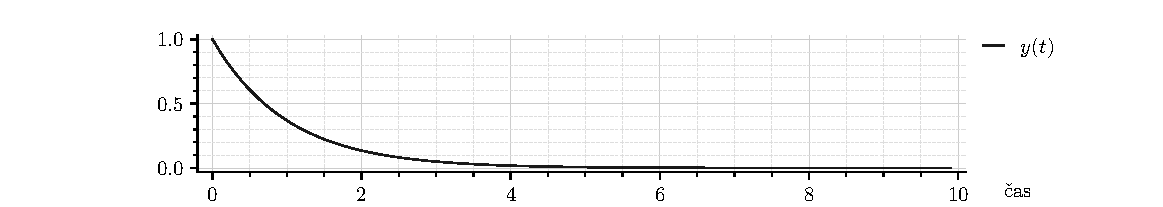
\includegraphics{ICH_SS1R_p1.pdf}
        }

        \figcaption{Impulzná charakteristika statického systému prvého rádu pre $a_0 = 1$ a $b_0 = 1$}
        \label{ICH_SS1R_p1}
    }%vbox

\end{center}



\subsection{ICH AS1R}
Časová funkcia \eqref{eq:ICH1R} bude impulznou charakteristikou astatického systému prvého rádu ak $a_0 = 0$. Na nasledujúcom obrázku je graf výslednej časovej funkcie

\begin{center}

    \vbox{%
        \makebox[\textwidth][c]{%
        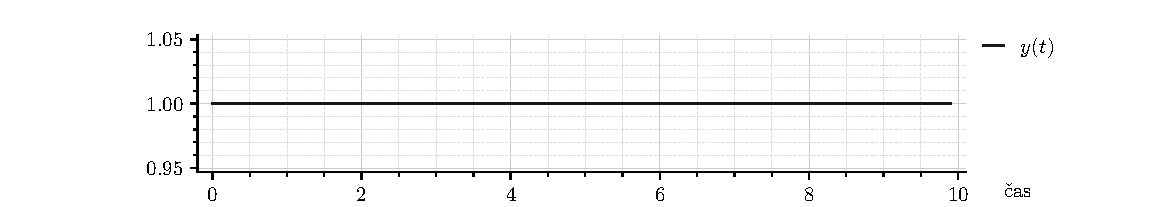
\includegraphics{ICH_AS1R_p1.pdf}
        }

        \figcaption{Impulzná charakteristika statického systému prvého rádu pre $a_0 = 0$ a $b_0 = 1$}
        \label{ICH_AS1R_p1}
    }%vbox

\end{center}


\subsection{ICH nestabilného systému prvého rádu}
Pre úplnosť uveďme aj prípad, keď $a_0 < 0$, teda systém je nestabilný. Zvoľme $a_0 = -1$. Na nasledujúcom obrázku je graf výslednej časovej funkcie

\begin{center}

    \vbox{%
        \makebox[\textwidth][c]{%
        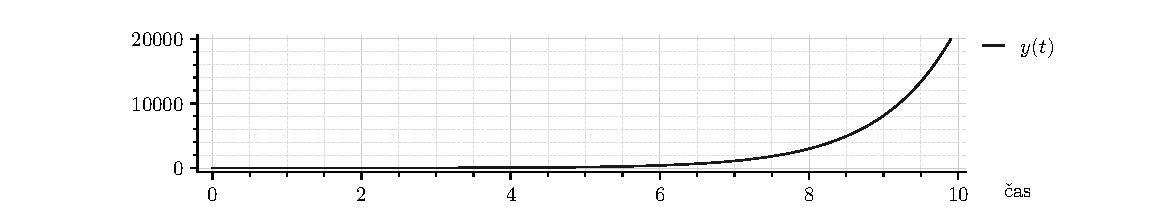
\includegraphics{ICH_unstable1R_p1.pdf}
        }

        \figcaption{Impulzná charakteristika statického systému prvého rádu pre $a_0 = -1$ a $b_0 = 1$}
        \label{ICH_unstable1R_p1}
    }%vbox

\end{center}





\section{Prechodová charakteristika}

Prechodová charakteristika je odpoveď systému na jednotkový skok.

\bigskip

Jednotkový skok je signál, ktorý je nulový pre $t < 0$ a má jednotkovú veľkosť pre $t \geq 0$. Ide o skokovú zmenu v čase $t=0$. Laplaceov obraz jednotkového skoku je $U(s) = \frac{1}{s}$.

Keďže máme k dispozícii matematický opis systému, prechodovú charakteristiku môžeme	nájsť analyticky. Prenosová funkcia systému prvého rádu je \eqref{eq:prvyradprenosovafunkcia}. Laplaceov obraz vstupného signálu je $U(s) = \frac{1}{s}$. Laplaceov obraz výstupného signálu potom bude
\begin{subequations}
\begin{align}
    Y(s) &= G(s) U(s) = \frac{b_0}{s + a_0} \frac{1}{s} \\
    Y(s) &= \frac{b_0}{s(s + a_0)}
\end{align}
\end{subequations}
Pre hľadanie originálu tohto obrazu je výhodné prepísať tento výraz na parciálny zlomok
\begin{subequations}
\begin{align}
    \frac{b_0}{s(s + a_0)} &= \frac{A}{s} + \frac{B}{s + a_0} \\
    b_0 &= A(s + a_0) + B s
\end{align}
\end{subequations}
kde $A$ a $B$ sú neznáme koeficienty. Uvedené platí pre akúkoľvek hodnotu $s$. Pre $s = 0$ dostaneme
\begin{subequations}
\begin{align}
    b_0 &= A a_0 \\
    A &= \frac{b_0}{a_0}
\end{align}
\end{subequations}
Pre $s = -a_0$ dostaneme
\begin{subequations}
\begin{align}
    b_0 &= B (-a_0) \\
    B &= -\frac{b_0}{a_0}
\end{align}
\end{subequations}
Obraz výstupného signálu je teda
\begin{equation}
    Y(s) = \frac{b_0}{a_0} \frac{1}{s} - \frac{b_0}{a_0} \frac{1}{s + a_0}
\end{equation}
a jeho originál
\begin{subequations}
\begin{align}
    y(t) &= \frac{b_0}{a_0} - \frac{b_0}{a_0} e^{-a_0 t} \\
    y(t) &= \frac{b_0}{a_0} \left(1 - e^{-a_0 t}\right)  \label{eq:PCH1Rfull}
\end{align}
\end{subequations}
čo je časová funkcia, ktorá je analytickým vyjadrením prechodovej charakteristiky systému. V uvedenom sme zjavne predpokladali, že $a_0 \neq 0$. 

Ak $a_0 = 0$, potom obraz výstupného signálu je
\begin{subequations}
\begin{align}
    Y(s) &= \frac{b_0}{s^2} \\
    Y(s) &= b_0 \frac{1}{s^2}
\end{align}
\end{subequations}
a jeho originál je
\begin{equation} \label{eq:PCH1Rint}
    y(t) = b_0 t
\end{equation}
čo je časová funkcia, ktorá je analytickým vyjadrením prechodovej charakteristiky systému ak $a_0 = 0$.



Je zrejmé, že pre prechodovú charakteristiku (PCH) je možné rozlišovať kvalitatívne rôzne prípady určené v tomto prípade jediným pólom systému. Pól systému je $s_1 = -a_0$.

V kontexte vyššie uvedeného možno rozlišovať prípady: statický systém prvého rádu (SS1R), astatický systém prvého rádu (AS1R) a nestabilný systém.






\subsection{PCH SS1R}

Časová funkcia \eqref{eq:PCH1Rfull} bude prechodovou charakteristikou statického systému prvého rádu ak $a_0 > 0$. Zvoľme $a_0 = 1$ a napríklad $b_0 = 1$. Na nasledujúcom obrázku je graf výslednej časovej funkcie

\begin{center}

    \vbox{%
        \makebox[\textwidth][c]{%
        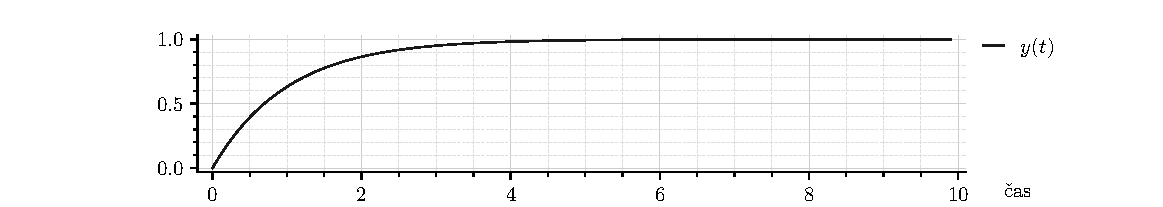
\includegraphics{PCH_SS1R_p1.pdf}
        }

        \figcaption{Prechodová charakteristika statického systému prvého rádu pre $a_0 = 1$ a $b_0 = 1$}
        \label{PCH_SS1R_p1}
    }%vbox

\end{center}



\subsection{PCH AS1R}

Časová funkcia \eqref{eq:PCH1Rint} bude prechodovou charakteristikou astatického systému prvého rádu ak $a_0 = 0$. Na nasledujúcom obrázku je graf výslednej časovej funkcie

\begin{center}

    \vbox{%
        \makebox[\textwidth][c]{%
        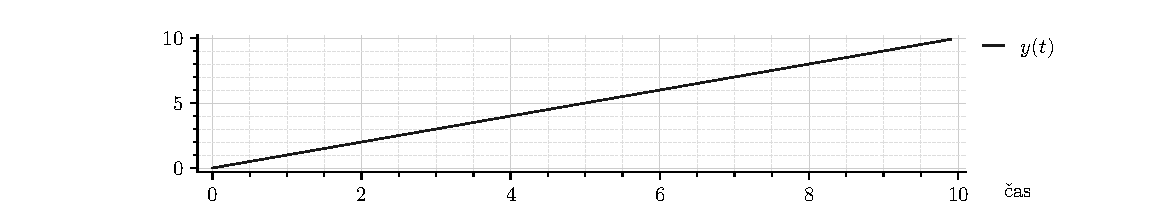
\includegraphics{PCH_AS1R_p1.pdf}
        }

        \figcaption{Prechodová charakteristika statického systému prvého rádu pre $a_0 = 0$ a~$b_0 = 1$}
        \label{PCH_AS1R_p1}
    }%vbox

\end{center}


\subsection{PCH nestabilného systému prvého rádu}

Pre úplnosť uveďme aj prípad, keď $a_0 < 0$, teda systém je nestabilný. Zvoľme $a_0 = -1$. Na nasledujúcom obrázku je graf výslednej časovej funkcie

\begin{center}

    \vbox{%
        \makebox[\textwidth][c]{%
        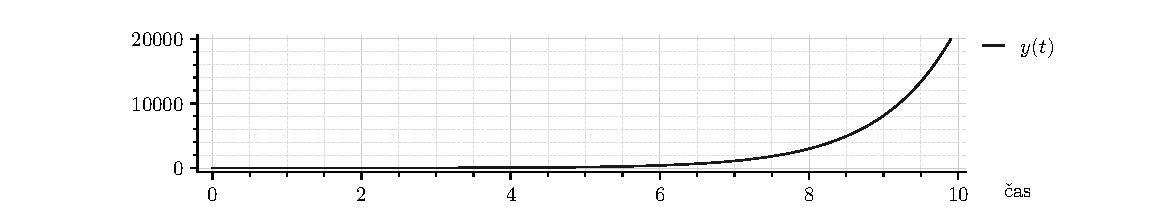
\includegraphics{PCH_unstable1R_p1.pdf}
        }

        \figcaption{Prechodová charakteristika statického systému prvého rádu pre $a_0 = -1$ a~$b_0 = 1$}
        \label{PCH_unstable1R_p1}
    }%vbox

\end{center}












\section{Prílohy}

V tejto časti sú prezentované skripty v programovacom jazyku Python, pomocou ktorých je možné nakresliť vyššie uvedené grafy impulzných a prechodových charakteristík. Skripty sú prezentované formou Jupyter notebooku a v nasledujúcich sekciách sú zobrazené jednotlivé bunky týchto notebookov

\subsection{Python skript pre vykreslenie grafov impulzných charakteristík}

\vbox{%
\begin{lstlisting}[language=Python, caption=Súbor \lstinline|../ICH1R.ipynb cell:02|]
import numpy as np
import matplotlib.pyplot as plt

# Parametre
b_0 = 1
a_0 = 1

# Súradnice bodov na x-ovej osi
plotData_x = np.arange(0, 10, 0.1)

# Výpočet hodnôt na y-ovej osi v zmysle danej časovej funkcie
plotData_y = b_0 * np.exp(-a_0 * plotData_x) \end{lstlisting}
}%end of vbox
\vbox{%
\begin{lstlisting}[language=Python, caption=Súbor \lstinline|../ICH1R.ipynb cell:03|]
# Kreslenie grafu
plt.plot(plotData_x, plotData_y)
plt.xlabel('čas $t$')
plt.ylabel('$y(t)$')
plt.show() \end{lstlisting}
\begin{center}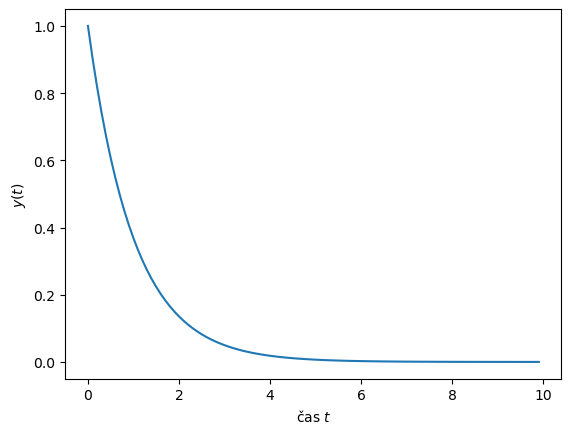
\includegraphics[width=0.68\textwidth]{ICH1Ripynb_cell03out.png}\end{center}}%end of vbox
\vbox{%
\begin{lstlisting}[language=Python, caption=Súbor \lstinline|../ICH1R.ipynb cell:04|]
# Obrázok pre hlavný text
figName = 'ICH_SS1R'
figNameNum = 0
exec(open('./figjobs/figJob_01.py', encoding='utf-8').read()) \end{lstlisting}
}%end of vbox
\vbox{%
\begin{lstlisting}[language=Python, caption=Súbor \lstinline|../ICH1R.ipynb cell:05|]
# Zmeňme hodnotu parametra a_0
a_0 = 0

# Výpočet hodnôt na y-ovej osi v zmysle danej časovej funkcie
plotData_y = b_0 * np.exp(-a_0 * plotData_x) \end{lstlisting}
}%end of vbox
\vbox{%
\begin{lstlisting}[language=Python, caption=Súbor \lstinline|../ICH1R.ipynb cell:06|]
# Kreslenie grafu
plt.plot(plotData_x, plotData_y)
plt.xlabel('čas $t$')
plt.ylabel('$y(t)$')
plt.show() \end{lstlisting}
\begin{center}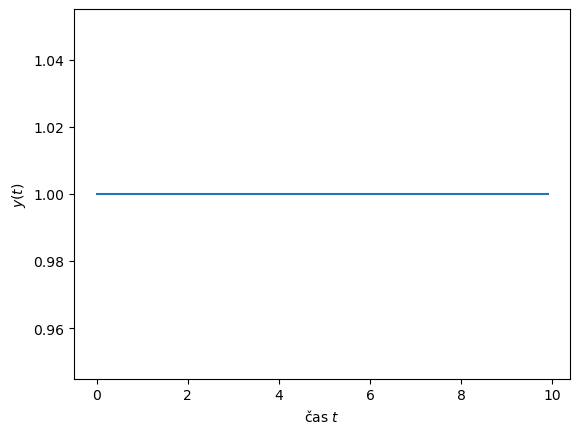
\includegraphics[width=0.68\textwidth]{ICH1Ripynb_cell06out.png}\end{center}}%end of vbox
\vbox{%
\begin{lstlisting}[language=Python, caption=Súbor \lstinline|../ICH1R.ipynb cell:07|]
# Obrázok pre hlavný text
figName = 'ICH_AS1R'
figNameNum = 0
exec(open('./figjobs/figJob_01.py', encoding='utf-8').read()) \end{lstlisting}
}%end of vbox
\vbox{%
\begin{lstlisting}[language=Python, caption=Súbor \lstinline|../ICH1R.ipynb cell:08|]
# Zmeňme hodnotu parametra a_0
a_0 = -1

# Výpočet hodnôt na y-ovej osi v zmysle danej časovej funkcie
plotData_y = b_0 * np.exp(-a_0 * plotData_x) \end{lstlisting}
}%end of vbox
\vbox{%
\begin{lstlisting}[language=Python, caption=Súbor \lstinline|../ICH1R.ipynb cell:09|]
# Kreslenie grafu
plt.plot(plotData_x, plotData_y)
plt.xlabel('čas $t$')
plt.ylabel('$y(t)$')
plt.show() \end{lstlisting}
\begin{center}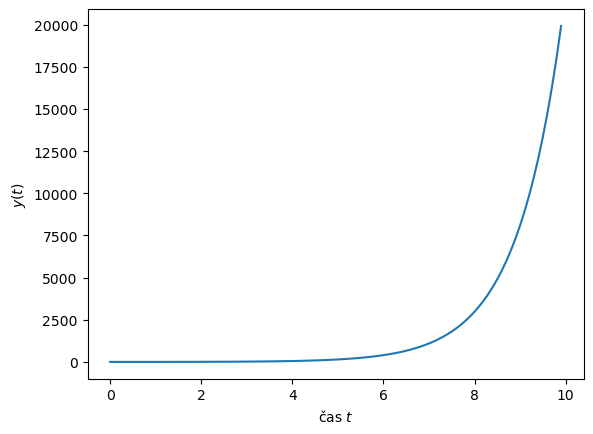
\includegraphics[width=0.68\textwidth]{ICH1Ripynb_cell09out.png}\end{center}}%end of vbox
\vbox{%
\begin{lstlisting}[language=Python, caption=Súbor \lstinline|../ICH1R.ipynb cell:10|]
# Obrázok pre hlavný text
figName = 'ICH_unstable1R'
figNameNum = 0
exec(open('./figjobs/figJob_01.py', encoding='utf-8').read()) \end{lstlisting}
}%end of vbox



\subsection{Python skript pre vykreslenie grafov prechodových charakteristík}

\vbox{%
\begin{lstlisting}[language=Python, caption=Súbor \lstinline|../PCH1R.ipynb cell:02|]
import numpy as np
import matplotlib.pyplot as plt

# Parametre
b_0 = 1
a_0 = 1

# Súradnice bodov na x-ovej osi
plotData_x = np.arange(0, 10, 0.1)

# Výpočet hodnôt na y-ovej osi v zmysle danej časovej funkcie
plotData_y = (b_0/a_0) * (1 - np.exp(-a_0 * plotData_x)) \end{lstlisting}
}%end of vbox
\vbox{%
\begin{lstlisting}[language=Python, caption=Súbor \lstinline|../PCH1R.ipynb cell:03|]
# Kreslenie grafu
plt.plot(plotData_x, plotData_y)
plt.xlabel('čas $t$')
plt.ylabel('$y(t)$')
plt.show() \end{lstlisting}
\begin{center}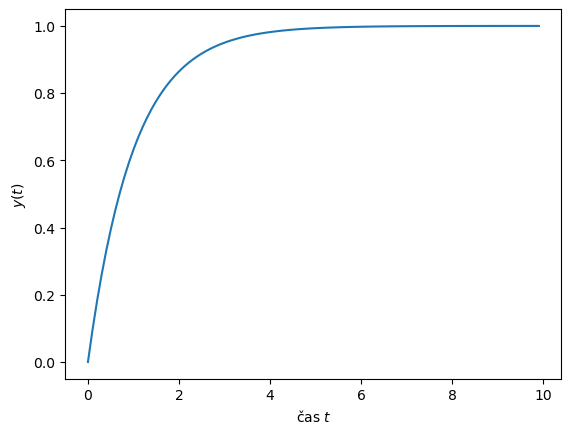
\includegraphics[width=0.68\textwidth]{PCH1Ripynb_cell03out.png}\end{center}}%end of vbox
\vbox{%
\begin{lstlisting}[language=Python, caption=Súbor \lstinline|../PCH1R.ipynb cell:04|]
# Obrázok pre hlavný text
figName = 'PCH_SS1R'
figNameNum = 0
exec(open('./figjobs/figJob_01.py', encoding='utf-8').read()) \end{lstlisting}
}%end of vbox
\vbox{%
\begin{lstlisting}[language=Python, caption=Súbor \lstinline|../PCH1R.ipynb cell:05|]
# Zmeňme hodnotu parametra a_0
a_0 = 0

# Výpočet hodnôt na y-ovej osi v zmysle danej časovej funkcie
plotData_y = b_0 * plotData_x \end{lstlisting}
}%end of vbox
\vbox{%
\begin{lstlisting}[language=Python, caption=Súbor \lstinline|../PCH1R.ipynb cell:06|]
# Kreslenie grafu
plt.plot(plotData_x, plotData_y)
plt.xlabel('čas $t$')
plt.ylabel('$y(t)$')
plt.show() \end{lstlisting}
\begin{center}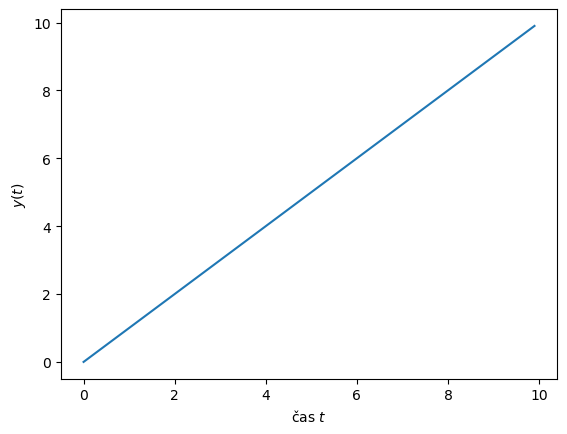
\includegraphics[width=0.68\textwidth]{PCH1Ripynb_cell06out.png}\end{center}}%end of vbox
\vbox{%
\begin{lstlisting}[language=Python, caption=Súbor \lstinline|../PCH1R.ipynb cell:07|]
# Obrázok pre hlavný text
figName = 'PCH_AS1R'
figNameNum = 0
exec(open('./figjobs/figJob_01.py', encoding='utf-8').read()) \end{lstlisting}
}%end of vbox
\vbox{%
\begin{lstlisting}[language=Python, caption=Súbor \lstinline|../PCH1R.ipynb cell:08|]
# Zmeňme hodnotu parametra a_0
a_0 = -1

# Výpočet hodnôt na y-ovej osi v zmysle danej časovej funkcie
plotData_y = (b_0/a_0) * (1 - np.exp(-a_0 * plotData_x)) \end{lstlisting}
}%end of vbox
\vbox{%
\begin{lstlisting}[language=Python, caption=Súbor \lstinline|../PCH1R.ipynb cell:09|]
# Kreslenie grafu
plt.plot(plotData_x, plotData_y)
plt.xlabel('čas $t$')
plt.ylabel('$y(t)$')
plt.show() \end{lstlisting}
\begin{center}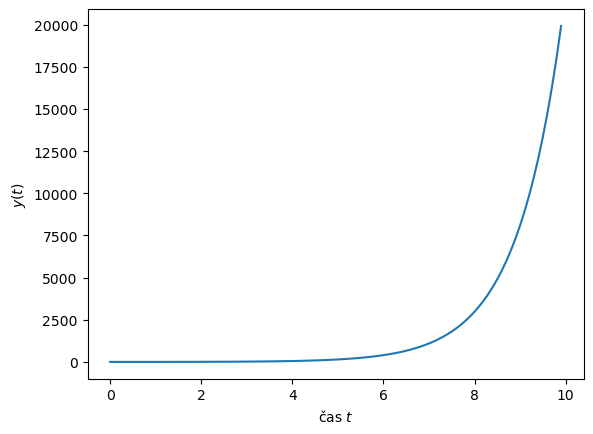
\includegraphics[width=0.68\textwidth]{PCH1Ripynb_cell09out.png}\end{center}}%end of vbox
\vbox{%
\begin{lstlisting}[language=Python, caption=Súbor \lstinline|../PCH1R.ipynb cell:10|]
# Obrázok pre hlavný text
figName = 'PCH_unstable1R'
figNameNum = 0
exec(open('./figjobs/figJob_01.py', encoding='utf-8').read()) \end{lstlisting}
}%end of vbox




















% -----------------------------------------------------------------------------

\end{document}

% -----------------------------------------------------------------------------